\documentclass[xcolor=dvipsnames]{beamer}

\usepackage{pdfpages} % for the code of conduct
\usepackage{todonotes}
\usepackage{graphicx}
\usepackage{hyperref}

% \PassOptionsToPackage{dvipsnames,svgnames,x11names}{xcolor}

\hypersetup{
    colorlinks = true,
    linkbordercolor = {red}
}

\title{\input{title.txt}}
\author{Markus A.G. Amano}
\subtitle{\href{https://inspirehep.net/literature/2690368}{ arXiv:2308.11686 (Amano, Kaminski et al. 2023) }
  % \\{\tiny accepted for publication with Progress in Particle and Nuclear Physics}
}
\institute{Yamagata University (as a JSPS Fellow)}


\begin{document}

{
\setbeamercolor{background canvas}{bg=}
\includepdf[pages=1]{codeofconduct.pdf}
}

\maketitle

\begin{frame}
  \frametitle{Two Motivating Questions}
  \begin{itemize}
    \item What is the hydrodynamic description of QCD in the Quark Gluon Plasma phase?
    \item How does vorticity affect Quark Gluon Plasma matter?
  \end{itemize}
  \missingfigure{Catchy Quark Gluon Plasma Graphic}
\end{frame}

\begin{frame}
  \frametitle{The Holographic Description}


  \begin{block}{Holographic Principle}
    The information of the universe can be encoded on its boundaries.
  \end{block}

  \begin{block}{}
    string theory + Maldacena $\longrightarrow$ AdS/CFT
  \end{block}

  \missingfigure{A graphic symbolizing AdS/CFT}

\end{frame}

\begin{frame}
  \frametitle{Conformal Field Theory}
  \framesubtitle{``the field theory side''}
  % CFT
  \begin{block}{}
    \alert{CFT}(conformal field theory) is a field thery that does not change under conformal transformations.
    $$\eta \rightarrow \Omega^2 \eta$$
  \end{block}

  \begin{block}{Conformal Transformations}
    \begin{itemize}
      \item Translations, 
      \item Rotations and Lorentz transformations
      \item \textbf{Dilations}
      \item \textbf{Special Conformal Transformations}
    \end{itemize}
  \end{block}

\end{frame}

\begin{frame}
  \frametitle{Anti de-Sitter Space}
  \framesubtitle{``the gravity side''}

  % AdS
  \begin{block}{}
    \alert{AdS}(Anti de-Sitter) is a negatively curved space that is as \textit{symmetric as} Minkowski space.
  \end{block}

  \begin{itemize}
    \item conformally flat 
      $ds^2 = \frac {L^2}{z^2} \left( -dt^2 + d\vec x\cdot d\vec x + dz^2 \right)$
    \item negative Curvature 
      $R = -20/L^2$
    \item classical gravity with matter fields
  \end{itemize}

  \missingfigure{Einstein Hilbert Action Action}
\end{frame}

% AdS/CFT
% Action Dictionary/Witten Relation

\begin{frame}
  \frametitle{A Holographic Description }
  \framesubtitle{(Gubser et al 1998, Witten 1998) [Textbook Natsuume 2012]}
  \begin{block}{GKP-Witten Relation}
    \begin{center}Z$_\text{gauge}$ = Z$_\text{AdS}$\end{center}
    $$\left\langle \exp\left(i\int\phi^{(0)} \mathcal O_\phi\right) \right\rangle =  e^{i S_\text{on-shell}[\phi(z\rightarrow0) = \phi^{(0)}]}$$
  \end{block}
  
  \begin{block}{The Holographic Dictionary}
    \begin{align*}
      \left\langle T_{\mu\nu}\right\rangle &\longleftrightarrow g_{\mu\nu}\\
      \left\langle J_{\mu}\right\rangle &\longleftrightarrow A_{\mu}\\
      \left\langle\mathcal O_\phi\right\rangle &\longleftrightarrow \phi
    \end{align*}
  \end{block}

  % put a column in the bottom if possible

\end{frame}

\subsection{Making a Dual State}

\begin{frame}
  \frametitle{Adding Temperature}

  \begin{block}{}Non-zero Temperature $\longleftrightarrow$ Event Horizon\end{block}

  \begin{block}{}
    $\frac {L^2}{z^2} \left( -dt^2 + d\vec x\cdot d\vec x + dz^2 \right) \rightarrow \frac {L^2}{z^2} \left( -f(z) dt^2 + d\vec x\cdot d\vec x + \frac 1{f(z)}dz^2 \right)$

    $ f(z) = 1 - z^3/z_h^2\,, \quad \mathrm T \propto 1/z_h $
  \end{block}

  \missingfigure{a figure that present temperature if possible}

\end{frame}

\begin{frame}
  \frametitle{Adding Rotating}
  \framesubtitle{at non-zero temperature}

  \begin{block}{}rotation $\longleftrightarrow$ event horizon that rotates relative to the boundary\end{block}

  \begin{block}{}
    $\frac {L^2}{z^2} \left( -dt^2 + d\vec x\cdot d\vec x + dz^2 \right) \rightarrow$ \\$(4+1)$D Myers-Perry AdS Black Hole (Hawking et al 1998)
  \end{block}

  \begin{alertblock}{global AdS vs local patch}
    In the rotating case, we begin with global AdS, implying spherical symmetry for both the horizon and the boundary theory.
  \end{alertblock}

  \missingfigure{Zooming into a rotating black hole image to show relation between local and global views.}

\end{frame}

% Angular momentum (and angular velocity)
% 5d two angular momentum, 4d one angular momentum

\begin{frame}[squeeze]
  \frametitle{Mapping 4D Rotation to 3D}
  \begin{itemize}
    \item Two independent planes of rotation in $4$D 
    \item Hopf Coordinates: 
      \begin{align*}
        &x=\cos\psi_H\sin \theta_H\,,&y=\sin \psi_H\sin \theta_H\\
        &z=\cos \phi_H\cos \theta_H\,,&w=\sin \phi_H\cos \theta_H
      \end{align*}
    \item Angular Momentum Vector $J = a\frac\partial{\partial\theta_H} + b\frac\partial{\partial\theta_H}$
  \end{itemize}
  \begin{columns}[t]
    \begin{column}{0.5\paperwidth}
      \href{https://markuspad.com/figures/axis_lines.html}{\includegraphics[height=0.45\paperheight]{genfigs/axis_lines.pdf}}
    \end{column}
    \begin{column}{0.5\paperwidth}
      \href{https://markuspad.com/figures/hopf_links.html}{\includegraphics[height=0.45\paperheight]{genfigs/hopf_links.pdf}}
    \end{column}
  \end{columns}
  % Interactive Versions here and here
\end{frame}

\section{Our Research}

\begin{frame}
  \frametitle{Our Research Goals}
  \framesubtitle{and what we did}
  \missingfigure{Add the goals}
\end{frame}

% Simplifying Angular Momentum Configuration and the axis-full Configuration
\begin{frame}[squeeze]
  \frametitle{Equal Angular Momentum Black Hole}
  \framesubtitle{A ``Simply Spinning'' Black Hole}

  \begin{block}{Enhanced Symmetry}
    There is enhanced the symmetry with $a=b$.
    \begin{center}$U(1)\times U(1) \longrightarrow SU(2)\times U(1)$ \end{center}
  \end{block}

  \begin{equation*}
    \begin{aligned}
      % d s^2=\frac 1{G(r)}{dr}^2-\left(\frac{r^2}{\ell^2}+1\right)dt^2&+\frac 14 r^2 \left((\sigma^1)^2+(\sigma^2)^2+(\sigma^3)^2\right) \\ &+\frac{2 \mu  }{r^2} \left(\frac a2 \sigma^3+dt\right)^2
      d s^2=\frac 1{G(r)}{dr}^2-\left(\frac{r^2}{\ell^2}+1\right)dt^2&+\frac 14 r^2 \left(\sigma^+ \sigma^- +\sigma^- \sigma^+ +(\sigma^3)^2\right) \\ &+\frac{2 \mu  }{r^2} \left(\frac a2 \sigma^3+dt\right)^2
    \end{aligned}
  \end{equation*}

  \begin{itemize}
    \item Cooridnates: $(t, \theta, \phi, \psi, r)$
    \item $\sigma$'s for the metric of a 3D sphere
    \item $r_+ \equiv$ outer horizon, $\left(G(r_+)=0\right)$
    \item Angular momentum Vector $a\frac\partial{\partial\psi}$
  \end{itemize}

\end{frame}

\subsection{Metric Perturbations}

\begin{frame}
  \frametitle{Perturbing Field Theory}
  \framesubtitle{with metric perturbations [Reference Wald 1984 pg. 183]}

  \begin{block}{Perturbed Metric}
    \begin{equation*}
      g^{p}_{\mu\nu} {dx}^\mu {dx}^\nu = \left(g_{\mu\nu}+\epsilon~h_{\mu\nu}+O(\epsilon^2)\right) {dx}^\mu {dx}^\nu
    \end{equation*}

    \begin{equation*}
      \left\langle \delta T_{\mu\nu}\right\rangle\longleftrightarrow h_{\mu\nu}
    \end{equation*}
  \end{block}

  \begin{block}{Einstein Field Equations at First Order}
    \begin{equation*}
      -\frac{1}{2}\nabla_\mu \nabla_\nu h-\frac{1}{2}\nabla^\lambda \nabla_\lambda h_{\mu\nu}+\nabla^\lambda \nabla_{(\mu}h_{\nu)\lambda} = \textcolor{red}{\frac{2\Lambda}{D-2}h_{\mu\nu}}
    \end{equation*}
  \end{block}

  % The Einstein Field Equations at first order ([Wald 1984][wald1984]) are linear PDEs.

  \begin{block}{Enhanced Symmetry}
    \begin{center}PDEs $\rightarrow$ Decoupled set of ODEs\end{center}
  \end{block}

\end{frame}

\begin{frame}
  \frametitle{Perturbation Metric Decomposition}

  \begin{align*}
    % h_{\mu\nu} = \int d\omega e^{-i\omega t} \sum_{\mathcal{J} = 0} \sum_{\mathcal{M}=\mathcal{-J}}^{\mathcal{J}} \sum_{\mathcal{K'}=-(\mathcal{J}+2)}^{\mathcal{J}+2} h_{i j}(r,\omega, \mathcal{J},\mathcal{M},\mathcal{K}') \sigma^i_{\mu} \sigma^j_{\nu} D_{\mathcal{K'}-Q(\sigma^{i})-Q(\sigma^{j}) \mathcal{M}}^\mathcal{J}
    h_{\mu\nu} = \int d\omega e^{-i\omega t} \sum_{\mathcal{J}, \mathcal{K}', \mathcal{M}} h_{i j}(r,\omega, \mathcal{J},\mathcal{M},\mathcal{K}') \sigma^i_{\mu} \sigma^j_{\nu} D_{\mathcal{K'}-Q(\sigma^{i})-Q(\sigma^{j}) \mathcal{M}}^\mathcal{J}
  \end{align*}

  \begin{itemize}
    \item $\mathcal{J} > 0$, $-\left( \mathcal J + 2 \right) \leq \mathcal{K}' \leq \mathcal J + 2$, $-\mathcal J \leq \mathcal{M}'  \leq \mathcal J$
    \item $i, j \in \{t,r,3,+, -\}$
  \end{itemize}

  \begin{block}{$Q$, Eigenfunction}
    \alert{$Q$} is the angular momentum quantum charge of $\sigma^i$ and eigenfunction of $W_3 := i\partial_\psi$

    \begin{equation*}
      Q(\sigma^i) = 0 \text{ if } i=r,t,3;\quad 1 \text{ if } i=+;\quad -1 \text{ if } i=- 
    \end{equation*}
  \end{block}

\end{frame}

\begin{frame}
  \frametitle{Decomposition Facts}
  \framesubtitle{plugging the decomposed perturbation in to its equations of motion}

  \begin{itemize}
    \item $((\mathcal J, \mathcal M), \mathcal K')$ perturbations decouple
    \item $\mathcal M$ vanishes from equations
  \end{itemize}

  \missingfigure{figure to help split sectors}
\end{frame}

% Near Boundary Expansion
% Source/VEV
% Sourcless Perturbations -> Non-Hermitian Operator -> Quasinormal Modes -> Dual Spectrum
% Hydrodynamics
% Hydroydnamics Expansion
% Critical Point (Maybe)

\section{Results}

\begin{frame}{Results}

\href{https://arxiv.org/abs/2308.11686}{Amano, Kaminski et al.}

\begin{itemize}
\item
  Non-Hydrodynamic Modes and the effects of non-extremal rotation.
  \begin{itemize}
  \item
    Tensor
  \item
    Vector
  \item
    Scalar
  \end{itemize}
\item
  Cross Spectrum Comparison
\item
  The Emergence of Hydrodynamics
\item
  Stability
\end{itemize}
\end{frame}

\begin{frame}{\(\mathcal K' = \mathcal J + 2\) Tensor Sector}
  \missingfigure{\(\mathcal K' = \mathcal J + 2\) Tensor Sector Animation}
% \phantomsection\label{mathcal-k-mathcal-j-2-tensor-sector}
% \begin{center}
%     \animategraphics[loop,autoplay,width=0.8\textwidth]{10}{build/tensor_dance_v2-}{0}{121}
% \end{center}
\(\mathcal K' = \mathcal J + 2\); \(h_{++}\)
\end{frame}

\begin{frame}{\(\mathcal K' = \mathcal J + 1\) Vector Fluctuations}
  \begin{columns}[T]
    \begin{column}{0.33\textwidth}
      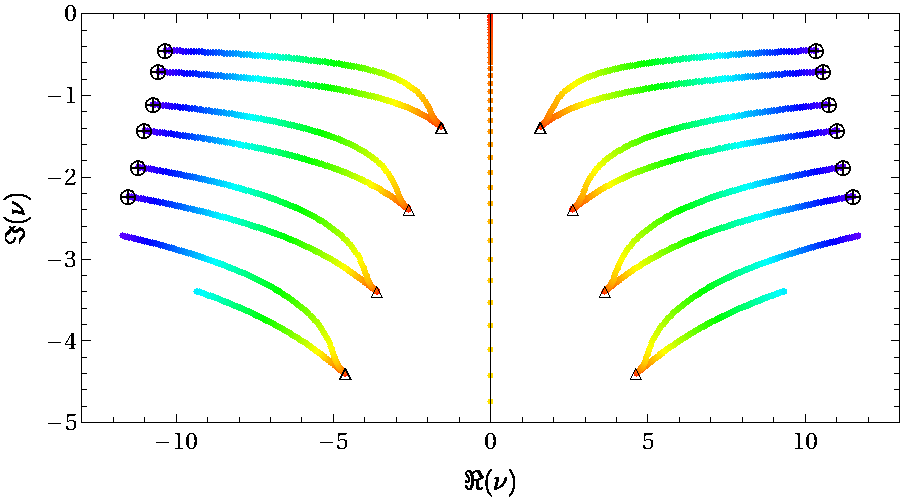
\includegraphics[width=1.05\textwidth]{figs/Vector_rp_10_grid_45_a_0.pdf}
    \end{column}

    \begin{column}{0.33\textwidth}
      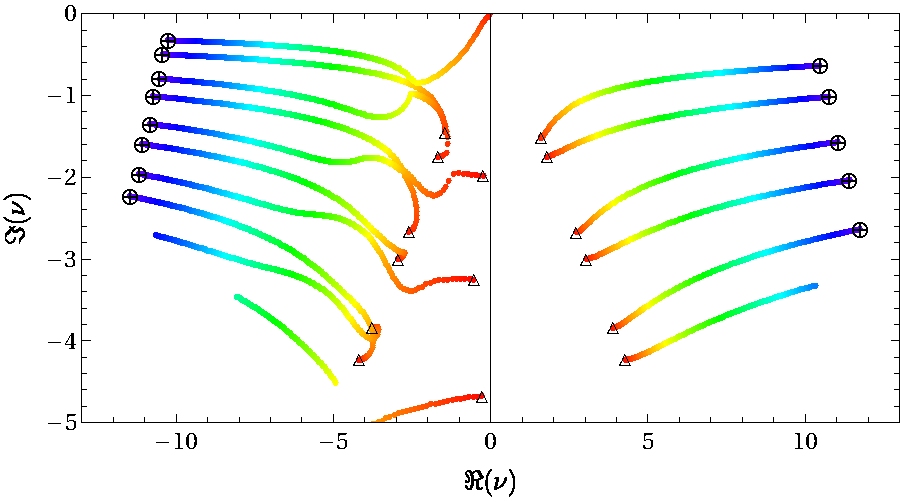
\includegraphics[width=1.05\textwidth]{figs/Vector_rp_10_grid_45_a_1_2.pdf}
    \end{column}

    \begin{column}{0.33\textwidth}
      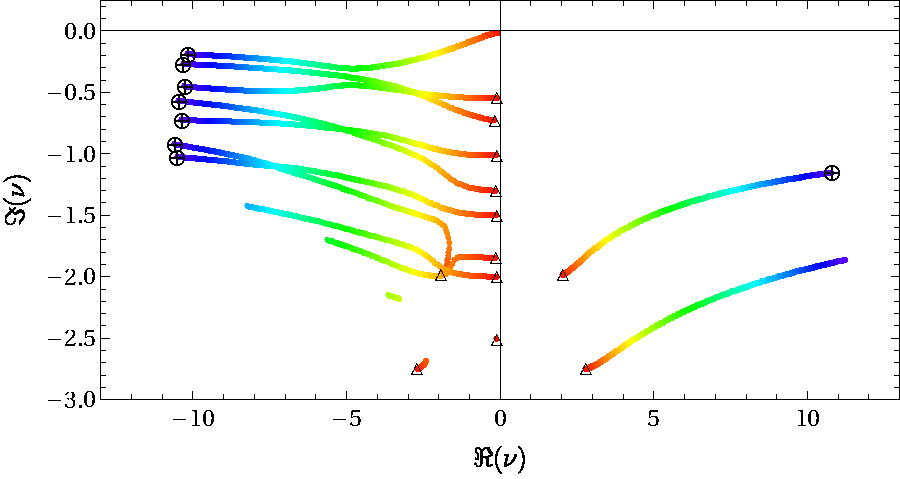
\includegraphics[width=1.05\textwidth]{figs/Vector_rp_10_grid_45_a_9_10.pdf}
    \end{column}
  \end{columns}

  \vfill

  \begin{columns}[c]
    \begin{column}{0.5\textwidth}
      \(a/\ell \in \{0, 1/2, 9/10\}\)\\
      \(\mathcal K' = \mathcal J + 1\); \(h_{+r}\), \(h_{+t}\), \(h_{+3}\) 
      (and \(h_{++}\) if \(\mathcal J \geq 1\))
    \end{column}

    \begin{column}{0.5\textwidth}
      \(\mathcal J = 0, 1/2, 1, \ldots, 199/2, 100\), \(r_+/\ell = 10\)\\
      \(\bigtriangleup \equiv \mathcal J = 0\),
      \(\bigoplus \equiv \mathcal J = 100\)
    \end{column}
  \end{columns}
\end{frame}

\begin{frame}{\(\mathcal K' = \mathcal J\) Scalar Fluctuations}

  \begin{columns}[T]
    \begin{column}{0.33\textwidth}
      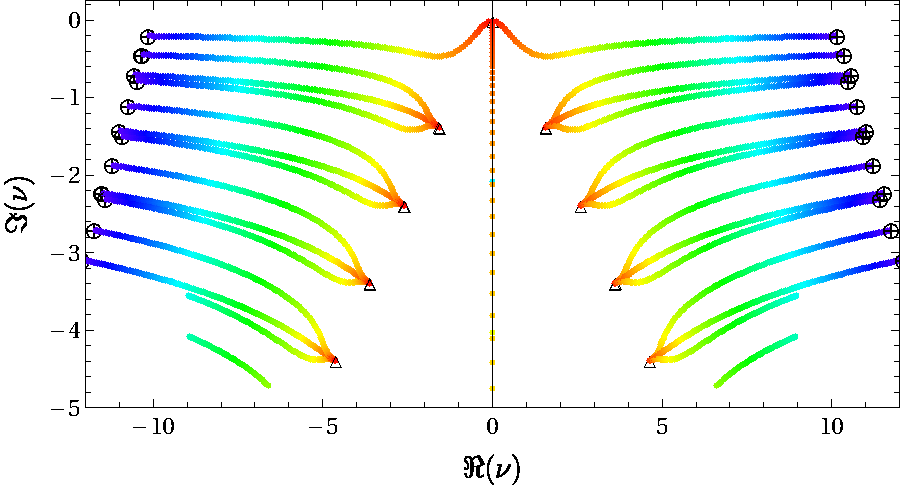
\includegraphics[width=1.05\textwidth]{figs/scalar_ef_spherical_a0.pdf}
    \end{column}

    \begin{column}{0.33\textwidth}
      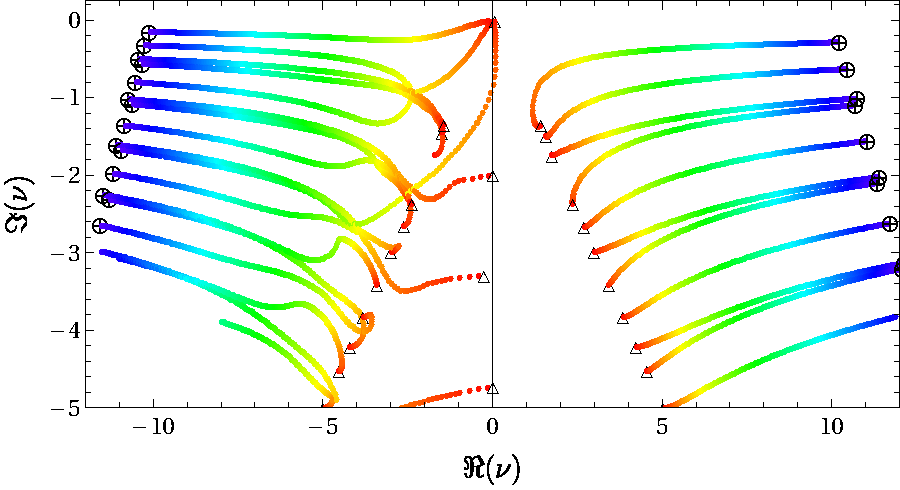
\includegraphics[width=1.05\textwidth]{figs/scalar_ef_spherical_a1_2.pdf}
    \end{column}

    \begin{column}{0.33\textwidth}
      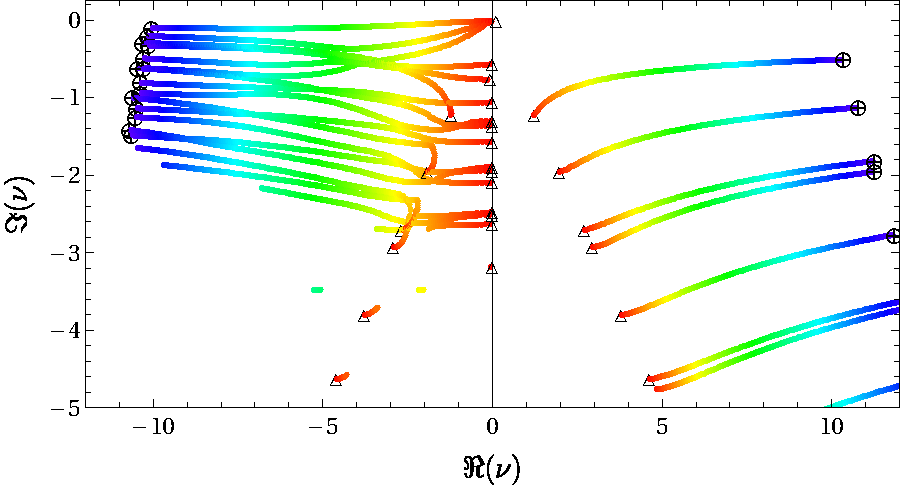
\includegraphics[width=1.05\textwidth]{figs/scalar_ef_spherical_a9_10.pdf}
    \end{column}
  \end{columns}

  \vfill

  \begin{columns}[c]
    \begin{column}{0.5\textwidth}
      \(a/\ell \in \{0, 1/2, 9/10\}\)\\
      \(\mathcal K' = \mathcal J\), \(h_{+-}\); \(h_{ab}\) where
      \(a,b \in \{r,t,3\}\)\\
      (, \(h_{+r}\), \(h_{+t}\), \(h_{+3}\) if \(\mathcal J \geq 1\) ) (, and
      \(h_{++}\) if \(\mathcal J \geq 2\))
    \end{column}

    \begin{column}{0.5\textwidth}
      \(\mathcal J = 0, 1/2, 1, \ldots, 199/2, 100\), \(r_+/\ell = 10\)\\
      \(\bigtriangleup \equiv \mathcal J = 0\),
      \(\bigoplus \equiv \mathcal J = 100\)
    \end{column}
  \end{columns}
\end{frame}

\begin{frame}{The Emergence of Hydrodynamics}
  To study the dispersion relations of the lowest gapless modes, we looked
  at the momentum diffusion sector.

  \vfill

  We solved spectra for
  \(r_+ = \{10, 100, 1000, 10^4 , 10^5 , 10^6 , 10^7 \}\) and
  \(\mathcal J = 0, 1/2, 1, \ldots, \mathcal J_\mathrm{max}\).\footnote<.->{\(\mathcal J_\mathrm{max}/r_+ = \mathit j_\mathrm{max} = 0.1\)}

  \vfill

  To see the emergence of hydrodynamics, we fitted the data to the
  equation below with fitting parameters \(\alpha\), \(\beta\), \(D\), and
  \(v\).

  \vfill

  \begin{equation}
    \omega = v \mathcal J^\beta - i D \mathcal J^\alpha
  \end{equation}
\end{frame}

\begin{frame}
  \begin{columns}[c]
    \begin{column}{0.5\textwidth}
      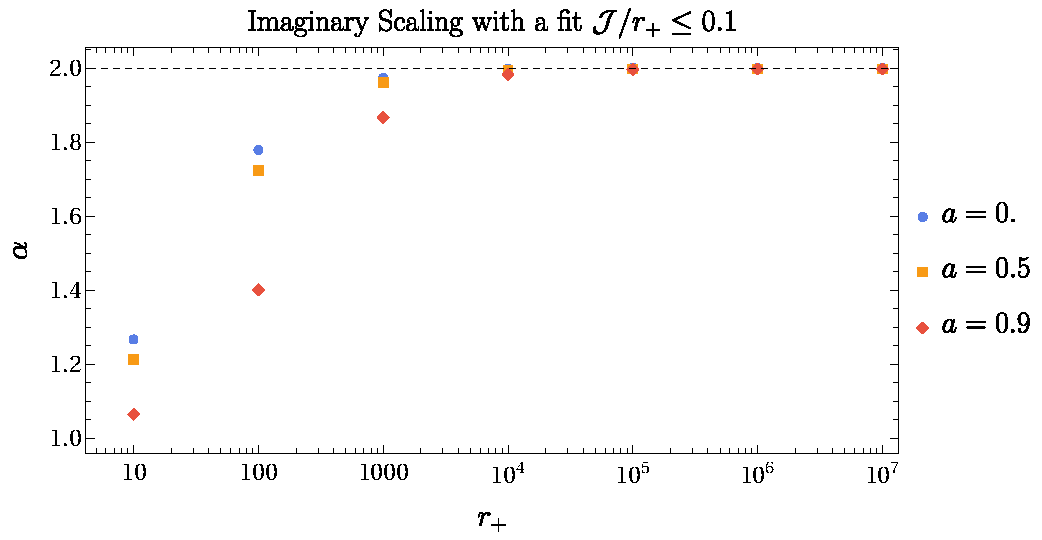
\includegraphics[width=1.05\textwidth]{figs/vector_dispersive_mode_rp_vs_im_scaling_over_a_scaled_Jleq0_1.pdf}\\
      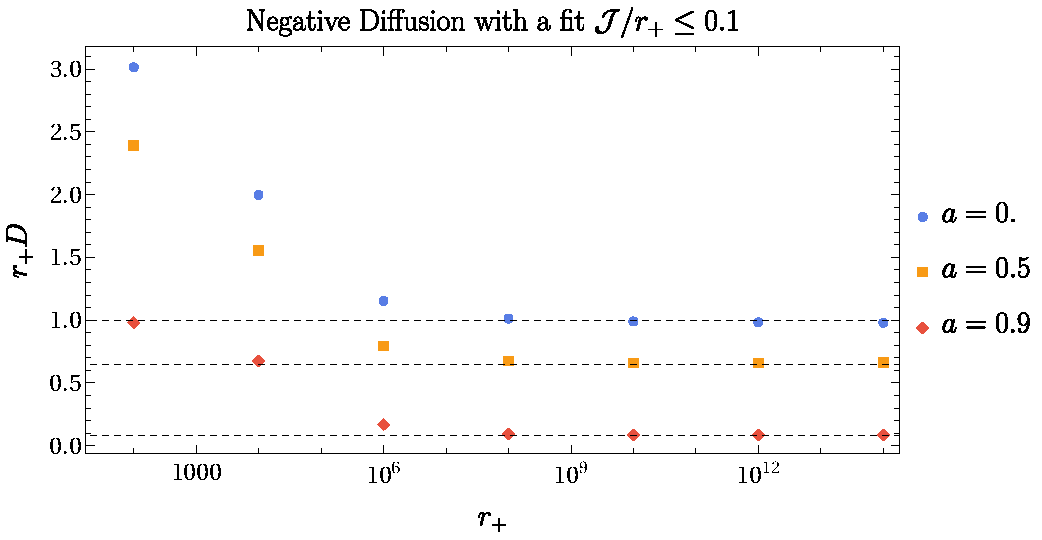
\includegraphics[width=1.05\textwidth]{figs/vector_dispersive_mode_rp_vs_diffusion_over_a_scaled_Jleq0_1.pdf}
    \end{column}

    \begin{column}{0.5\textwidth}
      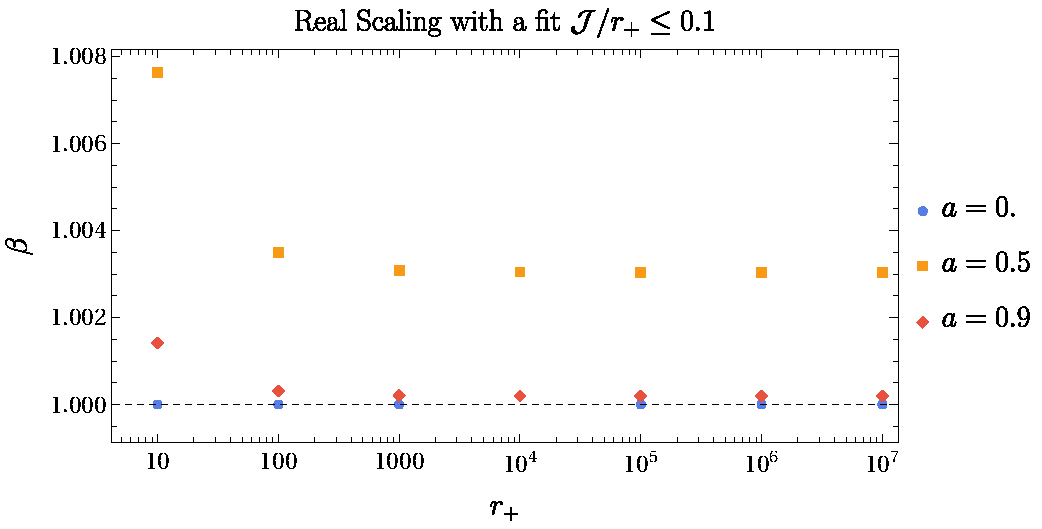
\includegraphics[width=1.05\textwidth]{figs/vector_dispersive_mode_rp_vs_re_scaling_over_a_scaled_Jleq0_1.pdf}\\
      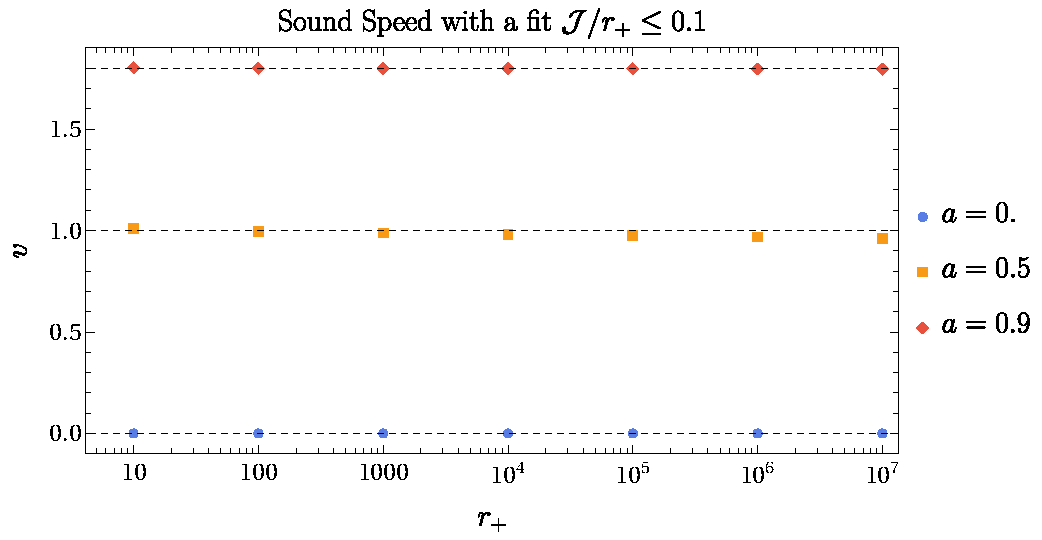
\includegraphics[width=1.05\textwidth]{figs/vector_dispersive_mode_rp_vs_soundspeed_over_a_scaled_Jleq0_1.pdf}
    \end{column}
  \end{columns}

  \vfill

  \begin{columns}[c]
    \begin{column}{0.5\textwidth}
      (\href{https://inspirehep.net/literature/1744607}{Kovtun 2019})
    \end{column}

    \begin{column}{0.5\textwidth}
      \begin{equation}
        \omega = v \mathcal J^\beta - i D \mathcal J^\alpha
      \end{equation}
    \end{column}
  \end{columns}
\end{frame}

\begin{frame}{Cross Spectrum Comparisons}
  \begin{columns}[T]
    \begin{column}{0.5\textwidth}
      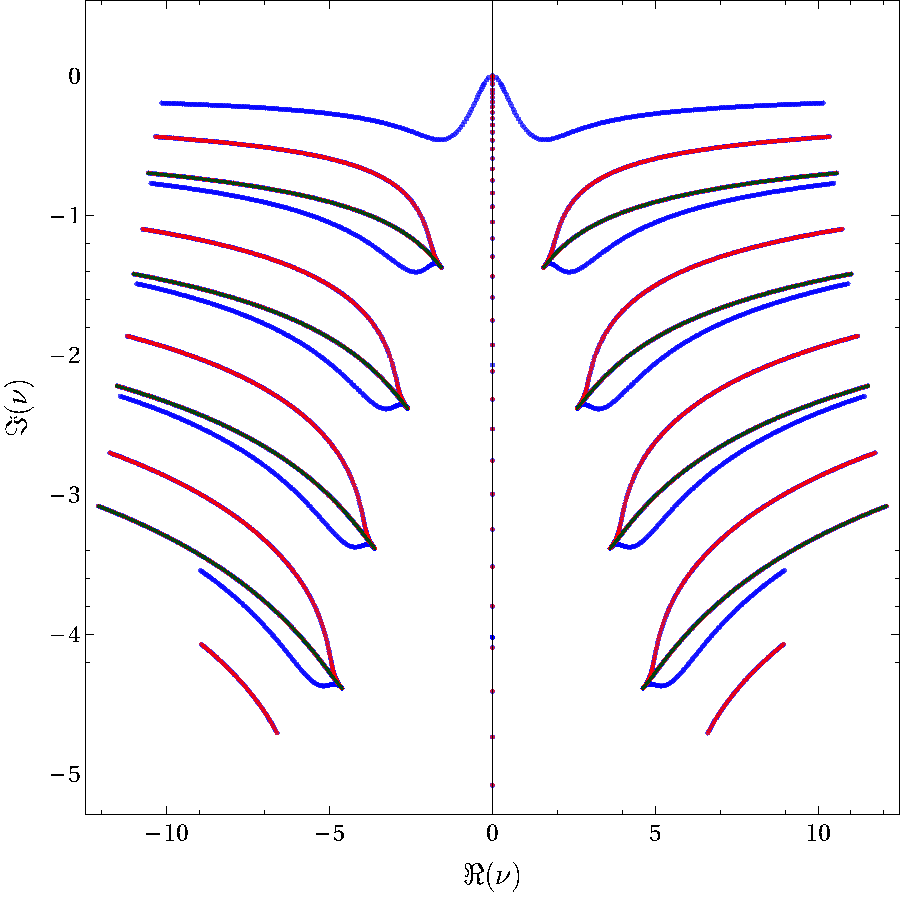
\includegraphics[width=0.9\textwidth]{figs/all_sectors_compared_ef_spherical_over_a0.pdf}
    \end{column}

    \begin{column}{0.5\textwidth}
      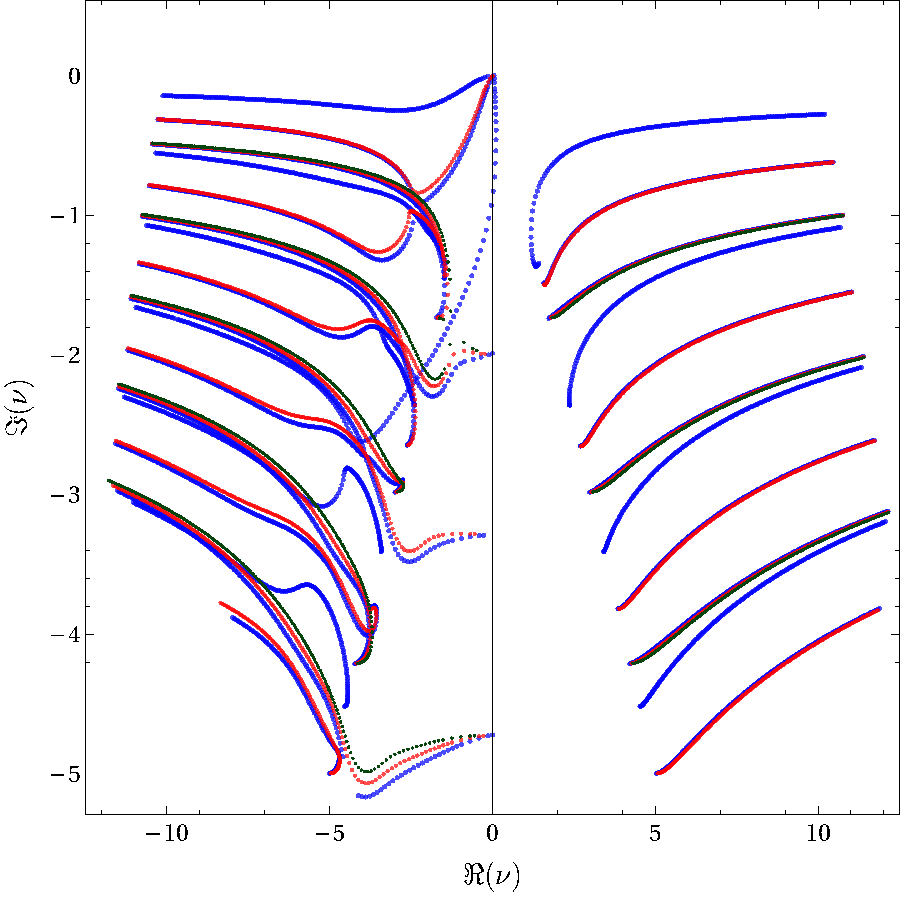
\includegraphics[width=0.9\textwidth]{figs/all_sectors_compared_ef_spherical_over_a1_2.pdf}
    \end{column}
  \end{columns}

  \vfill

  \begin{columns}[c]
    \begin{column}{0.33\textwidth}
      \textcolor{ForestGreen}{$\cdot$ Tensor}
    \end{column}

    \begin{column}{0.33\textwidth}
      \textcolor{red}{$\cdot$ Vector}
    \end{column}

    \begin{column}{0.33\textwidth}
      \textcolor{blue}{$\cdot$ Scalar}
    \end{column}
  \end{columns}
\end{frame}

\section{Conclusion}

\begin{frame}{Summary and Outlook}

  \begin{block}{Outlook}
    \begin{itemize}
      \item
        Look to calculate with a more general parameter space where
        \(\mathcal J_\phi\neq\mathcal J_\psi\) (\(a\neq b\)).

        \begin{itemize}
          \item
            No ``axis of rotation'' in current background.
          \item
            Need to solve 2 Variable PDE (\href{https://inspirehep.net/literature/1780844}{Amado et
            al 2020}, \href{https://inspirehep.net/literature/1844790}{Amado et
            al.~2021})
        \end{itemize}
      \item
        Different \textbf{sources} of rotation?

        \begin{itemize}
          \item
            Vector graviton sourcing the rotation $\sim$ 
            \(H_{\theta i} \sim \Omega_i r^2\)
          \item
            RN with magnetic field, \(A_\theta \sim \Omega_i r^2\)
            \href{https://inspirehep.net/literature/854786}{Domenech et
            al.~2010}
        \end{itemize}
      \item
        Interpretation of linear instability in the dual field theory?
      \item
        be used in ``hydro codes''
      \item
        Expand on the dynamics of $SU(2)\times U(1)$ \ldots RFP!
    \end{itemize}
  \end{block}

\end{frame}

\begin{frame}{Acknowledgements}

  This research was conducted with funding from the \emph{Postdoctoral
  Fellowship at Henan University}.

  \vfill 

  I would like to thank my collaborators, \emph{Matthias Kaminski},
  \emph{Casey Cartwright}, and \emph{Jackson Wu}, on yet another fruitful
  for the research presented in this presentation.

  \vfill 

  Research in this presentation also included contributions from

  \begin{itemize}
    \item
      \emph{Mike Blake}, \emph{Casey Cartwright}, \emph{Matthias Kaminski},
      and \emph{Anthony Thompson}\\
      \href{https://inspirehep.net/literature/2174613}{Amano et al.~2022}
    \item
      \emph{Casey Cartwright}, \emph{Matthias Kaminski}, \emph{Jorge
      Noronha}, \emph{Enrico Speranza}\\
      \href{https://inspirehep.net/literature/1994753}{Cartwright et
      al.~2023}
  \end{itemize}
\end{frame}

% Explain Tree

% CFT
% AdS
% AdS/CFT
% Action Dictionary/Witten Relation
% AdS Black Hole
% Temperature
% AdS MP AdS Black Hole
% Angular momentum (and angular velocity)
% 5d two angular momentum, 4d one angular momentum
% Simplifying Angular Momentum Configuration and the axis-full Configuration
% Linear Perturbations
% Near Boundary Expansion
% Source/VEV
% Sourcless Perturbations -> Non-Hermitian Operator -> Quasinormal Modes -> Dual Spectrum
% Hydrodynamics
% Hydroydnamics Expansion
% Critical Point (Maybe)

% Research Motivations
% rotating fluids are ubiquitous 
% Heavy-Ion Collisions at RHIC possess large vorticity
% The holography offers a microscopic to derive an equation of state
% Rotating black holes in holography are dual an equilibrated rotating fluid
% Perturbing the geometry is equivalent to perturbing the fluid allowing for hydrodynamic description the said fluid

% Any Temperature Results
% Multiple intersting qualities found of strongly rotating fluids
% - multiple level crossings
% - charge of charged fluids are similar angular momentum of spining fluids
% - confining phase has an instability
% Large Temperature Hydrodynamics Results
% - the rotating is dual to the boast
% - hydrodynamic transport coefficients
% - linearly stable
% - pole skipping points

% Keep the audience in mind both when preparing your talk and when presenting.
% The Rising Researchers Seminars are aimed at a broad nuclear theory audience.
% So you should assume that your audience has a good strong physics foundation,
% but you cannot assume that they know any particular nuclear physics detail
% beyond undergraduate physics, since they will all have pursued different
% graduate studies, learning different specific techniques and engaging with
% different tangential physics fields. In addition, remember that this series
% often has experimentalists in the audience.

% Provide a broad introduction that sets up the problem or question your research
% is addressing. Aim to provide a broad enough introduction that every audience
% member will feel they have understood in order to lay a strong foundation for
% the specifics of your research. Remember, it’s important to include the
% motivation for your research in the broader nuclear context, i.e., tell the
% audience why they should spend the next 40 min. listening to your talk instead
% of catching up on sleep.

% Don’t fall into the trap of thinking something is “too basic” to explain. We
% often feel that we are explaining something too basic and that the established
% senior researchers in the audience will be bored. This is a false impression,
% you can ask any of them. The less mental energy expended trying to recall
% “basic” concepts from the last time they taught it 20 years ago, the more
% energy they’ll have for understanding your actual research.

% Avoid jargon and acronyms. This is one of the biggest pitfalls for junior and
% senior researchers alike. If you do need to use them in your talk, always
% define them before you use them, even if they seem common. It’s generally good
% practice to remind your audience of the definition throughout the talk,
% particularly if it was defined early in your talk.

% Consider your color schemes carefully. One in twelve men are color blind (1 in
% 200 women). This is predominantly a red/green deficiency, so try not to use red
% and green in the same plot or text block. Here is a good resource to understand
% this better and get some ideas for workarounds. Also try to avoid any of the
% standard green, cyan, and magenta colors on a white background as they do not
% project well, even for people who are not color blind.

\end{document}
